\chapter{A review of the literature}

\section{Flow induced vibrations}
\label{sec:flow induced vibrations}


\section{Fluid-elastic galloping}
\label{fluid-elastic galloping}

Fluid-elastic galloping is one of the most commonly observable flow-induced vibration on a slender body. Since this phenomenon is most common in civil structure, such as buildings and iced-transmission lines, the term ``aeroelastic galloping" is commonly used as the body is immersed in air. However, this mechanism can occur on a slender body immersed in any Newtonian fluid, provided that the conditions to sustain the galloping mechanism are satisfied. This work is based on a general Newtonian flow,thus the term `` fluid-elastic galloping" is used throughout this thesis.
   

\subsection{Excitation of galloping}
\label{exci-galloping}

When a bluff body moves along the transverse direction of the fluid flow, it generates a force along the transverse direction. This force, also known as the induced lift is a resultant of the velocity of the fluid and the motion of the body. When this body is attached to an oscillating system (i.e. a simple spring, mass and damper system), the induced lift becomes the periodic forcing of the system. Galloping is sustained  if the induced lift is in phase with the motion of the body. This could be explained further by using a square cross section as an example.

\begin{figure}[!h]
\setlength{\unitlength}{\textwidth}

  \begin{picture}(1,0.36)(0,0.74)
    
  \put(0.2,0.76){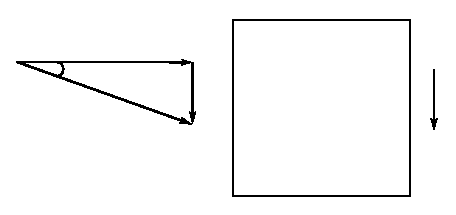
\includegraphics[width=0.5\unitlength]{./chapter-literature-revirw/fnp/setup-1.eps}}         
      
      
   
 	\put(0.315,1.04){$U$}
 	\put(0.3,0.95){$U_i$}
    \put(0.42,1.0){$\dot{y}$}
    \put(0.28,1.003){ $\theta$}
    \put(0.7,0.99){\small $(+)$}
      	

 	
 	 

     

  \end{picture}

 \caption{Induced angle of attack on a square prism due to the resultant of free-stream velocity of the fluid and transverse velocity of the body.}
    \label{fig:induced_lift_sketch}
\end{figure}

 Figure \ref{fig:induced_lift_sketch}  illustrates the motion of the body at a given instantaneous time.The induced angle of attack is formed on the square cross section as a result of the fressrteam velocity vector $U$ and the transverse velocity vector of the body $\dot{y}$. Thus, a force is formed in phase with the motion of the body (square cross section). This mechanism could also be observed on other bodies which are prone to galloping. The sign convention in this figure (and generally used in this scope of research) states that downward direction is positive. Hence, the force generated on a body under the influence of galloping, could be also identified as a ``negative lift".
 

\subsection{Qusasi-state theory}
\label{QSS theory}


According \cite{Paidoussis2010},the initial studies by \cite{Glauert1919} provided a criterion for galloping by considering the auto-rotation of a stalled aerofoil. As this phenomenon commonly occur in iced transmission lines, \cite{DenHartog1956} has provided a theoretical explanation for iced electric transmission lines. 

The pioneering study in order to mathematically model galloping was conducted by \cite{Parkinson1964}. This model has been widely used in almost all subsequent studies regarding galloping. A weakly non-linear oscillator model was developed by them to predict the response of the system. Essentially the quasi-steady assumption was made to develop this theory assuming that the instantaneous induced lift force of the oscillating body is equal to that of the lift force generated by the same body at the same induced angle of attack. In order to satisfy the quasi-steady assumption few conditions had to be satisfied.

\begin{itemize}
 \item The velocity of the body does not change rapidly
 \item There is no interaction between vortex shedding and galloping
\end{itemize}

The second condition is satisfied by ensuring the vortex shedding frequency is much higher than the galloping frequency.
The oscillator equation was solved using the Krylov and Bogoliubov method. Details of this method would not be mentioned as it is not used in the present study to solve the oscillator equation. The results obtained form experiments, carried out at $\reynoldsnumber=2200$ and a mass ratio (\mstar) around 1164 had a good agreement with the theoretical data which is shown in figure \ref{fig:parkinson_paper_data}.

\begin{figure}
	
  \setlength{\unitlength}{\textwidth}

        \begin{picture}(1,0.82)(0,0.4)

      % % % Parkinson Data 

      \put(0.05,0.39){\includegraphics[width=0.9\unitlength]{./chapter-literature-revirw/fnp/parkinson_data.eps}}
      
%       \put(0.07,0.95){$\displaystyle\frac{V}{D}$}
%       \put(0.07,1.3){$\displaystyle\frac{A}{D}$}
       \put(0.05,0.8){\Large$\frac{nA}{2\beta}\bar{Y}_s$}
       \put(0.52,0.42){\Large$\frac{nA}{2\beta}U$}
       \
%\put(0.189,1.415){\small(a)}
%\put(0.189,1.07){\small(b)}
%\put(0.189,0.73){\small(c)}

%  


    \end{picture}

  \caption{``Collapsed amplitude-velocity characteristic. Theory: \solidrule \ stable limit cycle, \dashedrule unstable limit cycle. Experiment $(\times) \ \beta = .00107$, $(\circ) \ \beta =.00196$,\ $(\vartriangle) \beta=.00364$,$(\triangledown) \ \beta = .00372$,\ $+1 \ \beta=.0012$,\ $+2 \ \beta=.0032$ Reynolds numbers $4,000-20,000$ ". Figure extracted from \cite{Parkinson1964}. $\frac{nA}{2\beta}\bar{Y}_s$ is the dimensionless displacement amplitude parameter and $\frac{nA}{2\beta}U$ is the reduced velocity.$\beta$ is the damping ratio and $n=\frac{1}{\mstar}$. The experimental data shows a good agreement with the theoretical model.}
    \label{fig:parkinson_paper_data}
\end{figure}

 %vspace{10cm}


\subsubsection*{Quasi-steady state oscillator model}

The equation of motion of transversely oscillating body is given by 
\begin{equation}
\label{equationofmotion}
m\ddot{y}+c\dot{y}+ky=F_y,
\end{equation}
where the forcing term $F_y$ is given by
\begin{equation}
\label{lift equation}
F_y=\frac{1}{2}\rho U^2\mathcal{A}C_y.
\end{equation}

As explained previously, when quasi-steady assumption is used the stationary $C_y$ data (which consists of both lift and drag data)  of the body could be could be used as inputs to the oscillator equation.\citet{Parkinson1964} used a $7^th$ order odd interpolating polynomial to determine $C_y$. The order of the polynomial can be chosen arbitrarily depending on the study. For example \citet{Barrero-Gil2009,Barrero-Gil2010a} have used a $3_{rd}$ order polynomial in order to simplify the analytical model. However, \citet{Ng2005} pointed out that a $7_{th}$ order polynomial is sufficient as it does not provide a significantly better result.    

\begin{equation}
\label{cy ploynomial}
C_y(\theta)=a_1\left(\frac{\dot{y}}{U}\right)-a_3\left(\frac{\dot{y}}{U}\right)^3+a_5\left(\frac{\dot{y}}{U}\right)^5-a_7\left(\frac{\dot{y}}{U}\right)^7.
\end{equation}

Therefore by substituting the forcing function to the oscillator equation (Eq:\ref{equationofmotion}) the Quasi-steady state (QSS) model could be obtained (Eq:\ref{final_equation_motion}). 

\begin{equation}
\label{final_equation_motion}
m\ddot{y}{+}c\dot{y}{+}ky{=}\frac{1}{2}\rho U^2 \mathcal {A} \Bigg(a_1\left(\frac{\dot{y}}{U}\right){-}a_3\left(\frac{\dot{y}}{U}\right)^3{+}a_5\left(\frac{\dot{y}}{U}\right)^5{-}a_7\left(\frac{\dot{y}}{U}\right)^7 \Bigg).
\end{equation}

As the current study is focused on the low \reynoldsnumber region, it is a known fact that the vortex shedding will be correlated well and therefore provide a significant forcing in the low Reynolds number region. \citet{Joly2012} introduced and additional sinusoidal forcing function to the model in order to integrate the forcing by vortex shedding. By the addition of this forcing \citet{Joly2012} managed to obtain accurate predictions of the displacement amplitude even at low mass ratios, where the galloping is suppressed or not present. Yet, the strength or the amplitude of this sinusoidal forcing has to be tuned in an \emph{ad hoc} manner, and it was not clear the relationship between this forcing with the other system parameters. Thus in the current study this forcing was not used.






\subsection{Induced force and the shear layers}

It is important to have an understanding on how the induced lift is generated in a fluid dynamics point of view. Since the quasi-steady model has already been validated and re-validated by many studies, the flow-field data of static body simulations of a square cross section, at different angle of attack is used as an example. 

% % % % % % % % % % % % % % %Put the shear layer explanation here % % % % % % % % % % % % %






















  


    

     










